\documentclass[tikz]{standalone}
\usepackage{amsmath,amssymb}
\usepackage{tikz}
\usetikzlibrary{positioning}
\usetikzlibrary{shapes,arrows} 

\tikzstyle{block} = [draw, fill=blue!20, rectangle, minimum height=3em, minimum width=4em]
\tikzstyle{controller} = [draw, fill=red!20, rectangle, minimum height=3em, minimum width=4em]
\tikzstyle{sum} = [draw, fill=blue!20, circle, node distance=1cm]
\tikzstyle{input} = [coordinate]
\tikzstyle{output} = [coordinate]

\begin{document}

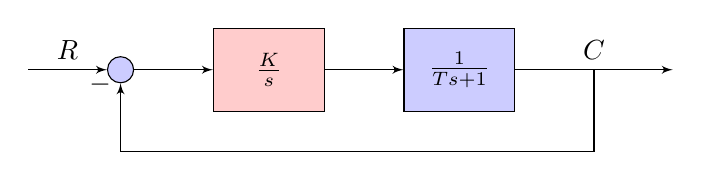
\begin{tikzpicture}[auto, >=latex']
% Nodes
\node [input] (input) {};
\node [sum, right = 1cm of input] (sum) {};
\node [controller, right = 1cm of sum] (system) {$\frac{K}{s}$};
\node [block, right = 1cm of system] (system2) {$\frac{1}{Ts+1}$};
\node [output, right = 2cm of system2] (output) {};
\node [input, below = 0.5cm of system] (m) {};
% Arrows
\draw [draw,->] (input) -- node {$R$} (sum);
\draw [->] (sum) -- node {} (system);
\draw [->] (system) --  (system2);
\draw [->] (system2) -- node (y) {$C$}(output);
\draw [-] (y) |- (m) {} ;
\draw [->] (m) -| node[pos=0.99] {$-$}  node [near end] {} (sum);
\end{tikzpicture}  
\end{document}